% THIS IS SIGPROC-SP.TEX - VERSION 3.1
% WORKS WITH V3.2SP OF ACM_PROC_ARTICLE-SP.CLS
% APRIL 2009
%
% It is an example file showing how to use the 'acm_proc_article-sp.cls' V3.2SP
% LaTeX2e document class file for Conference Proceedings submissions.
% ----------------------------------------------------------------------------------------------------------------
% This .tex file (and associated .cls V3.2SP) *DOES NOT* produce:
%       1) The Permission Statement
%       2) The Conference (location) Info information
%       3) The Copyright Line with ACM data
%       4) Page numbering
% ---------------------------------------------------------------------------------------------------------------
% It is an example which *does* use the .bib file (from which the .bbl file
% is produced).
% REMEMBER HOWEVER: After having produced the .bbl file,
% and prior to final submission,
% you need to 'insert'  your .bbl file into your source .tex file so as to provide
% ONE 'self-contained' source file.
%
% Questions regarding SIGS should be sent to
% Adrienne Griscti ---> griscti@acm.org
%
% Questions/suggestions regarding the guidelines, .tex and .cls files, etc. to
% Gerald Murray ---> murray@hq.acm.org
%
% For tracking purposes - this is V3.1SP - APRIL 2009

\documentclass{acm_proc_article-sp}

\begin{document}

\title{Structural Dissection of Business Entity Names}
%
% You need the command \numberofauthors to handle the 'placement
% and alignment' of the authors beneath the title.
%
% For aesthetic reasons, we recommend 'three authors at a time'
% i.e. three 'name/affiliation blocks' be placed beneath the title.
%
% NOTE: You are NOT restricted in how many 'rows' of
% "name/affiliations" may appear. We just ask that you restrict
% the number of 'columns' to three.
%
% Because of the available 'opening page real-estate'
% we ask you to refrain from putting more than six authors
% (two rows with three columns) beneath the article title.
% More than six makes the first-page appear very cluttered indeed.
%
% Use the \alignauthor commands to handle the names
% and affiliations for an 'aesthetic maximum' of six authors.
% Add names, affiliations, addresses for
% the seventh etc. author(s) as the argument for the
% \additionalauthors command.
% These 'additional authors' will be output/set for you
% without further effort on your part as the last section in
% the body of your article BEFORE References or any Appendices.

\numberofauthors{3} %  in this sample file, there are a *total*
% of EIGHT authors. SIX appear on the 'first-page' (for formatting
% reasons) and the remaining two appear in the \additionalauthors section.
%
\author{
% You can go ahead and credit any number of authors here,
% e.g. one 'row of three' or two rows (consisting of one row of three
% and a second row of one, two or three).
%
% The command \alignauthor (no curly braces needed) should
% precede each author name, affiliation/snail-mail address and
% e-mail address. Additionally, tag each line of
% affiliation/address with \affaddr, and tag the
% e-mail address with \email.
%
% 1st. author
\alignauthor
Venkatesh Vinayakarao\\
       \affaddr{Indraprastha Institute of Information Technology}\\
       \affaddr{New Delhi}\\
       \email{venkateshv@iiitd.ac.in}
% 2nd. author
\alignauthor
Srikanta Bedathur\\
       \affaddr{Indraprastha Institute of Information Technology}\\
       \affaddr{New Delhi}\\
       \email{bedathur@iiitd.ac.in}
% 3rd. author
\alignauthor
Amani Kongara\\
       \affaddr{Indraprastha Institute of Information Technology}\\
       \affaddr{New Delhi}\\
       \email{kongara1240@iiitd.ac.in}       
}
\date{20 Jan 2013}
% Just remember to make sure that the TOTAL number of authors
% is the number that will appear on the first page PLUS the
% number that will appear in the \additionalauthors section.

\maketitle
\begin{abstract}
Business entity (also known as local listing) names pose big challenge for search engines. Business entities like any other entity (people, place or product) appear to be unstructured at the outset and apparantly demonstrate human creativity. Our claim is that there are parts of these names that are recognizable and useful. We inspect 11,537 business entities from Phoenix, USA provided by the Yelp data set\footnote{http://www.yelp.com/dataset\_challenge/} towards gaining deep insights into how they are structured and if they can be annotated effectively. We argue about the characteristics of such names in detail including the opportunities and challenges in their annotation. An effort of this kind should lead to recommending a standard for capturing business names. A standard is much necessary in this domain since there are varied data providers and multiple search engines are consumers. Such a standard will alleviate the issues of record linkage, matching and ranking. In this process, we also make available, a manually tagged corpus of entity names for future research.
\end{abstract}

%A category including the fourth, optional field follows...
\category{H.3.3}{Information Storage and Retrieval}{Information Search and Retrieval}

\keywords{Tagging, Annotation, Normalization, Standardization} % NOT required for Proceedings

\section{Introduction}
Local search refers to the search of business in any specific place or their neighbourhoods. Let's say you are on the road and wish to locate the nearest seafood restaurant. In this case, you are doing a local search. With advances in mobile technologies and internet, local search has become indispensable. Business entity names play a significant role in the process of local search.

At the outset, business entity names seem to have no obvious structure. They are reflections of human creativity and the nature of business. We believe that a structural understanding of names will allow us to recognize, extract and normalize several of its parts. Most commercial search engines such as Google and Bing are known to buy foot-on-the-road entity data. Also, they may have their own proprietary systems to mine the web. Owing to existence of several such data sources (including prominent providers such as yelp and trip-advisor) and the variety in the way they capture the names, each entity gets morphed into several variants and that causes complications in record linkage, matching and ranking. For instance, consider, "Queen Elizabeth's Grammar School for Boys, Barnet, London". This is also known as "QE Boys", "QE Grammar School", "Queen Elizabeth's Grammar School" and "Queen Elizabeth's School". These are just few of the references to this school found on the web. An entity data provider may choose any of such ways to capture this entity, by name.

Towards a successful local search experience, its important to get a deep understanding of entity names. In this paper, we investigate the essential constituents of entity names and attempt to annotate them.


\section{Related Work}
There has been lot of work done on text document segmentation\cite{Beeferman:1999:SMT:309497.309507}\cite{Huang:2003:AML:945486.945492} and Query Segmentation \cite{Hagen:2011:QSR:1963405.1963423}\cite{Hagen:2010:PNQ:1835449.1835621}. Document segmentation typically looks at finding coherent sentences from textual documents typically through statistic, linguistic or probabilistic means. Query segmentation is much closer to our work since the text being segmented are short and have named entities in them. There has also been considerable work done on named entity recognition\cite{Guo:2009:NER:1571941.1571989}\cite{Li:2012:TNE:2348283.2348380} and linguistic processing of short text \cite{Murnane:2013:RLU:2487788.2488162}\cite{Taksa:2007:UWS:1262257.1262320}. However, the same techniques that work with queries do not work with entity names. For example, "My Sister Toy Shop" should lead to "My Sister" as the core name and "Toy Shop" as the category element. Most of the POS taggers will identify "My" as a Preposition which is not at all the case in this context. "A Stitch in Time" makes custom fit clothes. This name should not be split. Entire text, together, identifies the business.

Takahashi et al. \cite{Takahashi:2010:ETM:1884017.1884070}, analyze the truthfulness of modifiers such as "authentic", "impressive" in entity names. Oates et al.,\cite{Oates:2002:ULS:584931.584939} look for same entities in free text using LSA based approach. There has been several attempts at normalizing text such as gene name normalization\cite{Fang:2006:HGN:1567619.1567627}, person name normalization\cite{Magdy:2007:ACP:1654576.1654582} and location normalization \cite{Li:2002:LNI:1072228.1072355}. Business entity name normalization depends on these but is much more complicated since names could be a combination of person name, location, domain, etc.

Bouquet et al.,\cite{Bouquet:2008:ENS:1446294.1446425} proposed ENS (Entity Name System) to refer names uniformly. Their approach is to hash the names to uniform identifier. For example, "Paolo Bouquet" is referred to as "ok200706301185791252056" and is geared towards generation of such an identifier. One of their requirements is to maintain a large repository of global entity names. We take a different perspective of normalizing names. Our work could serve as a pre-processing step to this kind of normalization. While unique representation for a name happens to be the objective of Bouquet et al's approach, our approach works towards improving IR by extracting key elements of a name. 

Our work is to extract, re-organize and normalize the name parts. This does not always result in the same unique representation. Yet, this approach does generate semantically richer names. Humans can identify that "Nimbus American Bistro N' Brewery" refers to an entity whose name might be "Nimbus" or "Nimbus American" while belonging to "Bistro" and "Brewery" categories. We believe this can be learned and such names can be machine translated.

\section{Business Entity Name}
A typical entity name comprises of a core name along with various segments such as business categories and location. Since naming of an entity demands human creativity, there are several forms that an entity name can take. Essentially, we observed the entity name to contain these high level items:
\begin{enumerate}

\item Location: In "75th Thai Taste Restaurant", "75th" is part of the address and is followed by the core name "Thai Taste" whereas "Restaurant" is the category. The Location field may occur in the beginning or the later part along with the core name of an entity name.
\item CoreName:  The name, Scottsdale Medical Imaging LTD, has Scottsdale as the core name of the entity that distinguishes this entity from rest of the entities in the "Medical Imaging" domain. In the example "A Stitch in Time", the whole string is a core name. CoreName plays a huge role in identification of an entity and thus is a crucial component of entity name. In the manually annotated training set, we observed that 66\% of these CoreNames where either a God or Person.
\item Category: In "Every Kid's Dentist \& Orthodontics", "Every Kid's" is the core name of the entity which distinguishes it among the other entities of the categories, Dentists and the Orthodontics. In "Autohaus Service \& Performance Center", "Autohaus" is the core name, whereas "Service" \& "Performance Centre" is a category. Most of the entity names occur with the category to which it is associated.
\item Anchor: In "KC \& Co.", "KC" is the core name and "Co." is the anchor. Similarly in "Phoenix Paediatrics Ltd", "Phoenix" is the core name, "Paediatrics" is its domain and "Ltd" is its anchor word. HongKong's Company Naming Guideline \footnote{http://www.cr.gov.hk/en/publications/docs/name-e.pdf} says that these anchors ("Limited", "Company", "Company Limited", etc) will be ignored while checking if the companies are same.
\item Others: "R Bar at the Camelback Inn" contains the core name "R Bar", the connector "at" and the address "The Camelback Inn". We bucket such items that do not fall into any other recognizable part as "others".
\end{enumerate}
We wondered if there exist more ways of categorizing the parts of entity names. These parts came out of a 5 member survey on 100 names each. Each of them identified the parts in the similar way. As we see an entity name can be of any combination of these parts. Hence, their annotation is an interesting and challenging task.

\section{Names as Hidden Markov Model}
We visualize the words in entity name as a sequence of observed states. Behind each word, we visualize its category as its hidden state. We prepared the manually annotated training data with 500 randomly chosen entity names. A model thus generated was used with Viterbi decoding algorithm to predict the best possible hidden states, thereby, giving us the annotations.

\begin{figure}[!ht]
\begin{center}
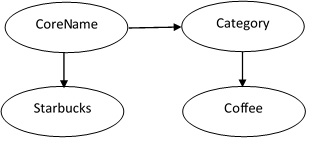
\includegraphics[scale=0.5]{namehmm.jpg}
\end{center}
\caption{
Visualization of our annotator as HMM
}
\label{figure1}
\end{figure}

The HMM is described with a state space S with initial probability pi, $x_i$ observed states and $y_i$ hidden states. In our case there are n  observed and hidden states where n is the number of tokens in the entity name. If $\alpha$ denotes the transition probability between states of S and k is the last state, the most likely state sequence is computed by viterbi method as
$$
V_{{t,k}} = {\mathrm  {P}}{\big (}y_{t}\ |\ k{\big )}\cdot \max _{{x\in S}} (a_{{x,k}}\cdot V_{{t-1,x}})
$$

\begin{figure}[!ht]
\begin{center}
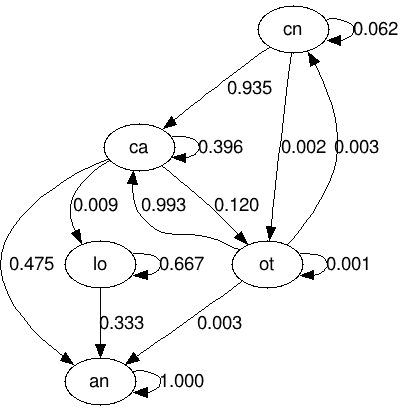
\includegraphics[scale=0.3]{probtrans.png}
\end{center}
\caption{
Transition probabilities between annotations from training data
}
\label{figure1}
\end{figure}

The transition probabilities learnt from manual annotations were very interesting. For instance, in all our examples, only anchor followed an anchor if at all there were multiple anchor terms. Hence the probability is 1. Category has even distribution for all transitions while corename shows a bias towards leading to categories. We believe these numbers are dependent on the culture and reflects what is considered as "most common". All our data belongs to businesses in Phoenix, USA.

\begin{table}[!ht]
\begin{center}
\begin{center}
  \begin{tabular}{ | l | r |}
    \hline
    Part & Precision \\ \hline 
    CoreName & 71\%  \\ \hline    
    Category & 82\% \\ \hline
    Location & 72\% \\ \hline 
  \end{tabular}
\end{center}
\end{center}
\caption{
Accuracy of HMM based annotations
}
\label{table}
\end{table}
Beyond an extent, precision could not be increased using training data. In the case of core names, the lack of precision attributed majorly to their abbreviations, acronyms, multi-language nature and varied positioning in the word sequence. This model seems to work fine with category much better than the rest. Categories, by nature are dictionary terms (such as school, university, hospital, mall, theatre, etc) and they repeat. Identifying category first and moving on to use this knowledge to fix the rest of the parts gave better results. Full list of country-specific anchors (such as pvt, ltd, co, inc, gmbh, etc) are available and hence could be hard-wired into our system. Hence all the evaluation results are given only for CoreName, Category and Location. Further, note that names can have multiple tokens as core name, category or location. For evaluation, we consider a result as precise only when all the manually judged corename tokens are identified as corename by this system. Same applies to location and category. For example, if judges have marked "Phoenix/CN Children's/CA Hospital/CA", we need the system to mark both Children's and Hospital tokens as category inorder to be counted as correct.  

\section{Boosting the HMM Results}
Along with HMM based name part detection, we observed following opportunities to boost precision:
\begin{enumerate}
\item URL Breaking: URLs give some indication of which part of the entity name is core name. For example, "Clearly Professional Window Cleaning" is www. cpwindowcleaning.com. Looking at several names, we can say that "window cleaning" is a popular category and "Clearly Professional" or "CP" is what uniquely identifies them. 
\item Address helps us resolve the location part of the name (if any) and also to detect LIE (location in entity). For example,"Vijayawada Public School, Vijayawada" is both an LIE as well as has location at the end, in its name.
\item "Arizona Auto Care" could be searched as "Arizona car care", "Arizona car service", "Arizona truck repair" and so on. There should be a way to extract these synonyms. A look at several companies in the auto care business allows us to capture a set of synonyms for "auto care". 
\item Abbreviations and Acronyms: BBQ, bnb, McD, Caltech, zoo vs zoological park. These can be found not only in core name but any part of the name. 
\item Name Breaking: PetSmart could be searched as "Pet Smart". We keep the investigation of related work on decompounding as future work. For now, we rely purely on capitalization.
\item Multi-Language nature - Its common to see chinese restaurants in India, Indian Restaurants in US and French restaurants everywhere!. Its fair to expect that the names will carry multiple languages. "Tortas El Guero", Gorditas El Tio are examples. 
\item Normalization: Each constituent needs to be normalized. For example, Mumbai and Bombay refer to same cities. "Satyam Computers" became "Tech Mahindra". Candidates for normalization also include words such as 'N, and, \& etc. For now, we have used a manual set of translations to normalize common words/phrases such as "and" for "'N", "BBQ" for "Barbeque" and so on. As future work, we leave creation of a synset for each part of the name and associate it to the normalized business name.
\end{enumerate}
For now, we used existing data from wikipedia and other internet sources to compile a supporting list of data such as location names, anchors and synonyms. This data was used to boost the hmm results. We observed a gain in precision as given in the table  below.
\begin{table}[!ht]
\begin{center}
\begin{center}
  \begin{tabular}{ | l | r |}
    \hline
    Part & Precision \\ \hline 
    CoreName & 77\%  \\ \hline    
    Category & 84\% \\ \hline
    Location & 83\% \\ \hline 
  \end{tabular}
\end{center}
\end{center}
\caption{
Accuracy of Boosted annotations
}
\end{table}

Some examples of the normalized text looks as follows:
\begin{table}
\begin{center}
  \begin{tabular}{ |p{2cm} | p{3cm} |}
    \hline
    Name & Annotated Name \\ \hline
    A Stitch in Time & A/CN Stitch/CN in/CN Time/CN   \\ \hline
    Scottsdale Medical Imaging LTD & Scottsdale/CN Medical/CA Imaging/CA LTD/AN  \\ \hline
    California Institute of Technology & California/CN Institute/CA of/CA Technology/CA \\ \hline
  \end{tabular}
\end{center}
\caption{Sample Annotations}
\end{table}

In the above table, annotations expand as follows: 
CN:CoreName, CA:Category, LO:location,  AN:Anchor, OT:Others.

\section{Conclusion and Future Work}
\cite{Vilain:2007:EEB:1614108.1614154} suggests with evidence that the existing name extraction approaches are not good enough. Our work should help such efforts. Moreover, the heuristics we looked at for boosting the results can be more elegantly modeled using markov logic networks. The training data that we used has 500 names with tags that are judged to be correct which is released for further research and we hope to build a bigger corpus.

Firstly and most importantly, it will be interesting to see the Precision, Recall and F-Scores for Learning to rank data sets when the annotations are available as additional features. Secondly, language issues in name need to be considered. We worked only with English names and names that have non-dictionary words as category were left out. Thirdly, we stopped with 2 levels of category description (domain, category) considering that we had only 11k items in our dataset. In real world datasets, the category ontology extraction will be a bigger challenge. There is also scope for improvement with spellers, word decompounders and location repositories. Multiple knowledge sources and non-local data can be used to improve entity identification\cite{vilain-huggins-wellner:2009:RANLP09}.

From this work, we believe a standard representation of entity names can be achieved and we showed one way of doing it with reasonable accuracy on the Yelp dataset.


%
% The following two commands are all you need in the
% initial runs of your .tex file to
% produce the bibliography for the citations in your paper.
\small
\bibliographystyle{abbrv}
\bibliography{sigproc}  % sigproc.bib is the name of the Bibliography in this case
% You must have a proper ".bib" file
%  and remember to run:
% latex bibtex latex latex
% to resolve all references
%
% ACM needs 'a single self-contained file'!
%
%APPENDICES are optional
%\balancecolumns

% This next section command marks the start of
% Appendix B, and does not continue the present hierarchy

\balancecolumns
% That's all folks!
\end{document}
